% DO NOT COMPILE THIS FILE DIRECTLY!
% This is included by the other .tex files.

\begin{frame}[t,plain]
\titlepage
\end{frame}

\colorlet{punct}{red!60!black}
\definecolor{background}{HTML}{EEEEEE}
\definecolor{delim}{RGB}{20,105,176}
\colorlet{numb}{magenta!60!black}

\lstdefinelanguage{brol}{
    basicstyle=\normalfont\ttfamily,
    numbers=left,
    numberstyle=\scriptsize,
    stepnumber=1,
    numbersep=8pt,
    showstringspaces=false,
    breaklines=true,
    frame=lines,
    basicstyle=\tiny,
    backgroundcolor=\color{background},
}


\begin{frame}[t, fragile]{Datasets used}
\begin{itemize}
        \item Eireann used Shodan stream of certificates (350k certificates in counting Bloomfilter).
                \begin{itemize}
                        \item Thanks to John (Shodan) Matherly.
                \end{itemize}
        \item Alex used the CIRCL Passive SSL datasets (around 100 millions certificates).
                \begin{itemize}
                        \item Thanks to GCHQ (for the idea).
                \end{itemize}
\end{itemize}
\end{frame}

\begin{frame}[t,fragile]{Problem statement}
        CSIRT or LIRT or security analysts have recurring issues to:
\begin{itemize}
        \item Find owners of IP addresses.
        \item Detect usage of CIDR blocks.
        \item Find vulnerable systems passively (and avoid intrusive scanning).
        \begin{itemize}
                \item Scale of potential impact.
        \end{itemize}
        \item Detect compromised services.
\end{itemize}
\end{frame}

\begin{frame}[t,fragile]{Acknowlegement}
        \begin{itemize}
                \item Thanks to GCHQ and the FLYING PIG program
                \item and Edward Snowden for releasing the document.
        \end{itemize}

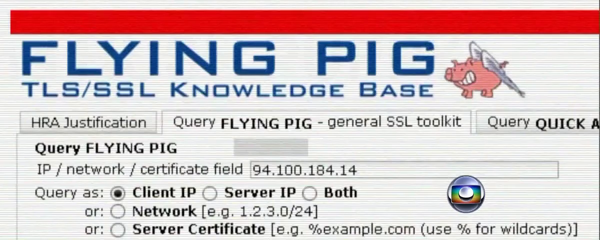
\includegraphics[scale=0.4]{FlyingPigHeader.png}
        \begin{itemize}
                \item Double edge techniques that can be used for good or bad reasons.
                \item Another opportunity to improve your threat modeling and your weak TLS knowledge.
        \end{itemize}
\end{frame}

\begin{frame}[t,fragile]{Passive SSL}
        \begin{itemize}
                \item Replicating Passive DNS concepts into SSL/TLS.
                \item Keeping a history of X.509 certificates seen per IP address.
                \begin{itemize}
                        \item Usage over time of the X.509 certificates.
                \end{itemize}
                \item Providing a search ReST interface per IP address, CIDR block.
                \item Tracing the use of CA and CRL/OCSP.
        \end{itemize}
\end{frame}

\begin{frame}[t,fragile]{Collecting X.509 Certificates - Internet Scanning}
        \begin{itemize}
                \item Scan the Internet yourself (e.g. In a single scan of the IPv4 space, close to 50 millions certificates).
                \item Which port to scan? protocol or service? pps?
                \item How often? (e.g. weekly scan helps to determine the stability of an IP,Certificate tuple)
                \item Cannot scan, you can reuse existing scanning data (e.g. \url{scans.io}).
        \end{itemize}
\end{frame}

\usetikzlibrary{positioning}

\begin{frame}[t,fragile]{Collecting X.509 Certificates - Passive DNS - SNI}
        \begin{itemize}
                \item On a single IPv4 address, you can have more than one certificate.
                        \begin{itemize}
                                \item Alternate SSL ports, multihomed systems
                                \item Other services: SSL-VPN, ESMTP, DTLS, IMAP, ...
                        \end{itemize}
                \item How to scan IPv6 address space for X.509 Certificates.
                \item Passive DNS used as a source for SNI (Server Name Indication) value or IPv6 addresses.
        \end{itemize}
        \tikzstyle{block} = [rectangle, draw, fill=green!20, text width=7em, text centered, rounded corners, minimum height=1.5em]
        \tikzstyle{line} = [draw, -latex']
        \begin{center}
        \scalebox{0.6}{
        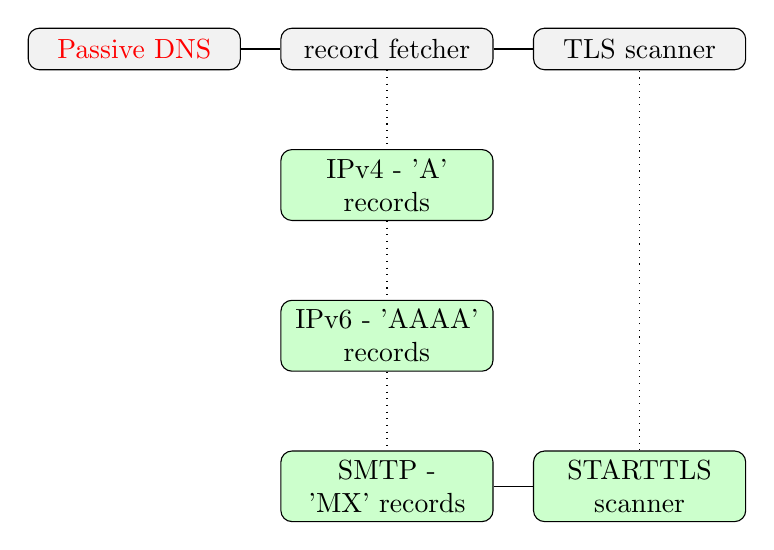
\begin{tikzpicture}[scale=1, node distance = 1cm and 5mm, auto, edge from parent/.style={->,draw}, >=latex]

        \node [block, fill=lightgray!20, text=red] (passivedns) {Passive DNS};
        \node [block, right = of passivedns, fill=lightgray!20] (domainextraction) {record fetcher};
        \node [block, below = of domainextraction] (Arecord) {IPv4 - 'A' records};
        \draw  [dotted] (domainextraction) -- (Arecord);
        \node [block, below = of Arecord] (AAAArecord) {IPv6 - 'AAAA' records};
        \draw [dotted] (Arecord) -- (AAAArecord);
        \node [block, below = of AAAArecord] (MXrecord) {SMTP - 'MX' records};
        \draw [dotted] (AAAArecord) -- (MXrecord);
        \node [block, right = of MXrecord] (STARTTLS) {STARTTLS scanner};
        \draw  (passivedns) -- (domainextraction);
        \node [block, right = of domainextraction, fill=lightgray!20] (scanner) {TLS scanner};
        \draw (MXrecord) -- (STARTTLS);
        \draw  (domainextraction) -- (scanner);
        \draw [dotted] (STARTTLS) -- (scanner);
        \end{tikzpicture}}
        \end{center}
\end{frame}

\begin{frame}[t,fragile]{Collecting X.509 Certificates - Network Interception}
\begin{itemize}
        \item Tapping a network interface where SSL/TLS handshakes are performed.
        \item TCP reassembly is still hard and finding SSL/TLS handshakes is a complementary problem.
        \item ssldump\footnote{\url{http://www.github.com/adulau/ssldump}}, Suricata, Moloch,...
        \item If you collect SSL/TLS handshakes in your internal network, don't forget the impact of intercepting proxies.
\end{itemize}
\end{frame}

\begin{frame}[t,fragile]{Collecting X.509 Certificates from Tor exit nodes}
\begin{itemize}
        \item Tor exit nodes traffic is an interesting source of alternative X.509 certificates (e.g. Tor circuits, XMPP sessions, TLS on non-standard ports).
        \item A huge proportion of flows uses TLS which provides a good overview of the most active X.509 certificates (e.g. Google, .vk.com...).
        \item Don't forget, not all the security researchers have good intention (e.g. FLYING PIG).
\end{itemize}
\end{frame}

\begin{frame}[t,fragile]{Security Perspective of X.509 Certificates}
\begin{itemize}
        \item Subject Name and Issuer Name can provide a lot of details about the devices, issuers or the overall security practices.
        \begin{itemize}
                \item A lot of X.509 certificates are automatically generated without the users knowledge.
                \item Detailed or sensitive information can leak in the X.509 certificate fields.
        \end{itemize}
\end{itemize}
          \begin{lstlisting}[language=brol]
4fd64e325ec7a14ac2e34bb5cfed28fef24c3ffb,C=DE, ST=Bavaria, L=Ingolstadt, O=Kaspersky Lab GmbH, OU=Pre-Sales, CN=rdg.klab.it.cx/emailAddress=consulting@kaspersky.de
dc4a127eae8a47a8041a4ce7f1a214c3e6957cd6,C=RU, ST=Moscow, L=Moscow, O=Kaspersky Lab ZAO, OU=IT, CN=nordnetsync.anti-theft.kaspersky.com
8a9c839f2ff275c79a985ea84b89bc9fa404d010,C=RU, ST=Moscow, L=Moscow, O=Kaspersky Lab, OU=IT, CN=owa.kaspersky.com
          \end{lstlisting}
\end{frame}

\begin{frame}[t,fragile]{Key-size distribution}
        \begin{center}
        \begin{tabular}{ l | c}
          Occurences&Key-size\\ \hline
          181899&1024\\
         143532&2048\\
         4997&512\\
         2845&4096\\
        1467&3072\\
        36&1023\\
     33&256\\
     30&2432\\
     26&768\\
     13&8192\\
     11&2047\\
     10&1536\\
        \end{tabular}
\end{center}

\end{frame}

\begin{frame}[t,fragile]{Key-size and Revocation}
        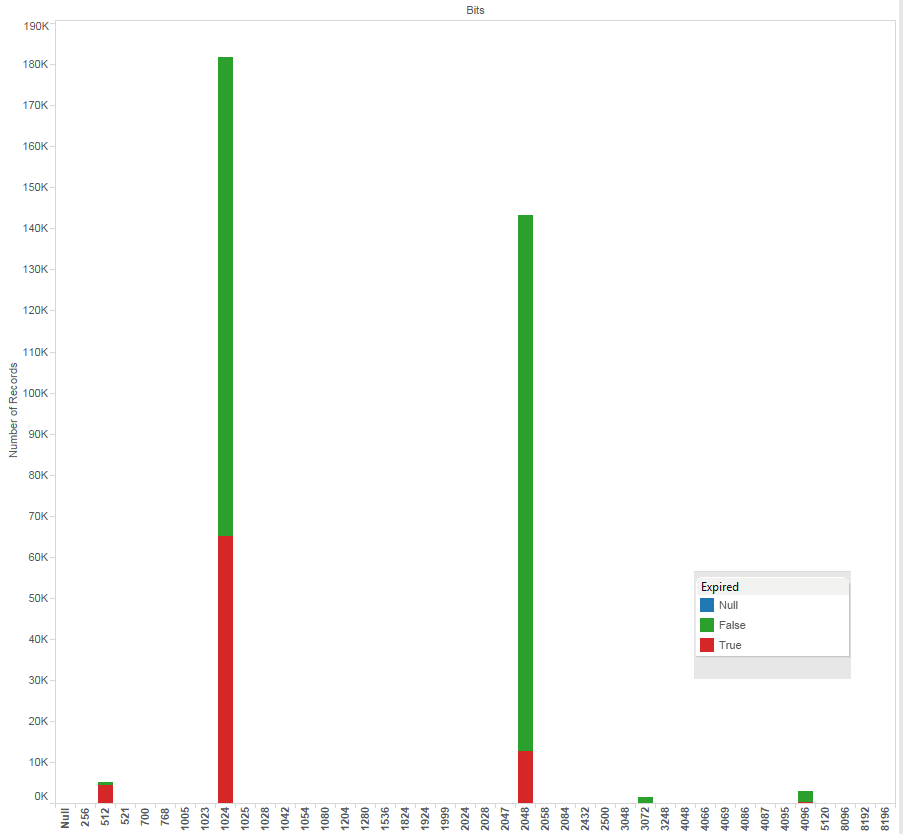
\includegraphics[scale=0.23]{./images/expired.png}
\end{frame}

\begin{frame}[t,fragile]{An Overview of Most Common Self-signed Certificates}
        \begin{center}
        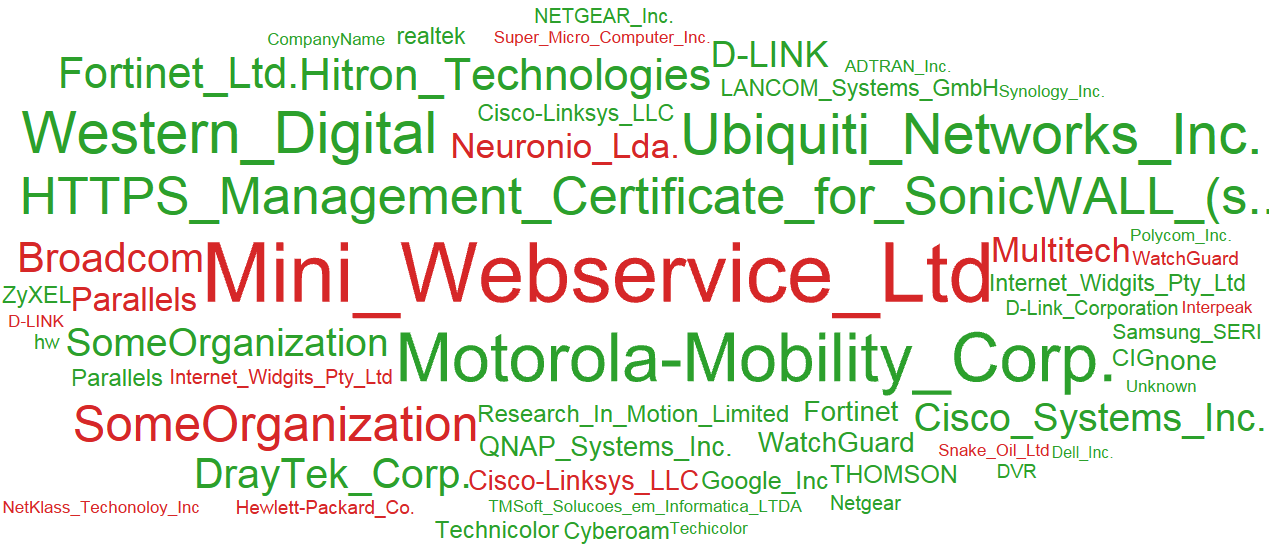
\includegraphics[scale=0.25]{./images/SelfSignedCloud.png}
        \end{center}
\end{frame}

\colorlet{punct}{red!60!black}
\definecolor{background}{HTML}{EEEEEE}
\definecolor{delim}{RGB}{20,105,176}
\colorlet{numb}{magenta!60!black}

\lstdefinelanguage{json}{
    basicstyle=\normalfont\ttfamily,
    numbers=left,
    numberstyle=\scriptsize,
    stepnumber=1,
    numbersep=8pt,
    showstringspaces=false,
    breaklines=true,
    frame=lines,
    backgroundcolor=\color{background},
    literate=
     *{0}{{{\color{numb}0}}}{1}
      {1}{{{\color{numb}1}}}{1}
      {2}{{{\color{numb}2}}}{1}
      {3}{{{\color{numb}3}}}{1}
      {4}{{{\color{numb}4}}}{1}
      {5}{{{\color{numb}5}}}{1}
      {6}{{{\color{numb}6}}}{1}
      {7}{{{\color{numb}7}}}{1}
      {8}{{{\color{numb}8}}}{1}
      {9}{{{\color{numb}9}}}{1}
      {:}{{{\color{punct}{:}}}}{1}
      {,}{{{\color{punct}{,}}}}{1}
      {\{}{{{\color{delim}{\{}}}}{1}
      {\}}{{{\color{delim}{\}}}}}{1}
      {[}{{{\color{delim}{[}}}}{1}
      {]}{{{\color{delim}{]}}}}{1},
}


\begin{frame}[t,fragile]{Most Common Subject and Org Names in X.509}
        \begin{center}
                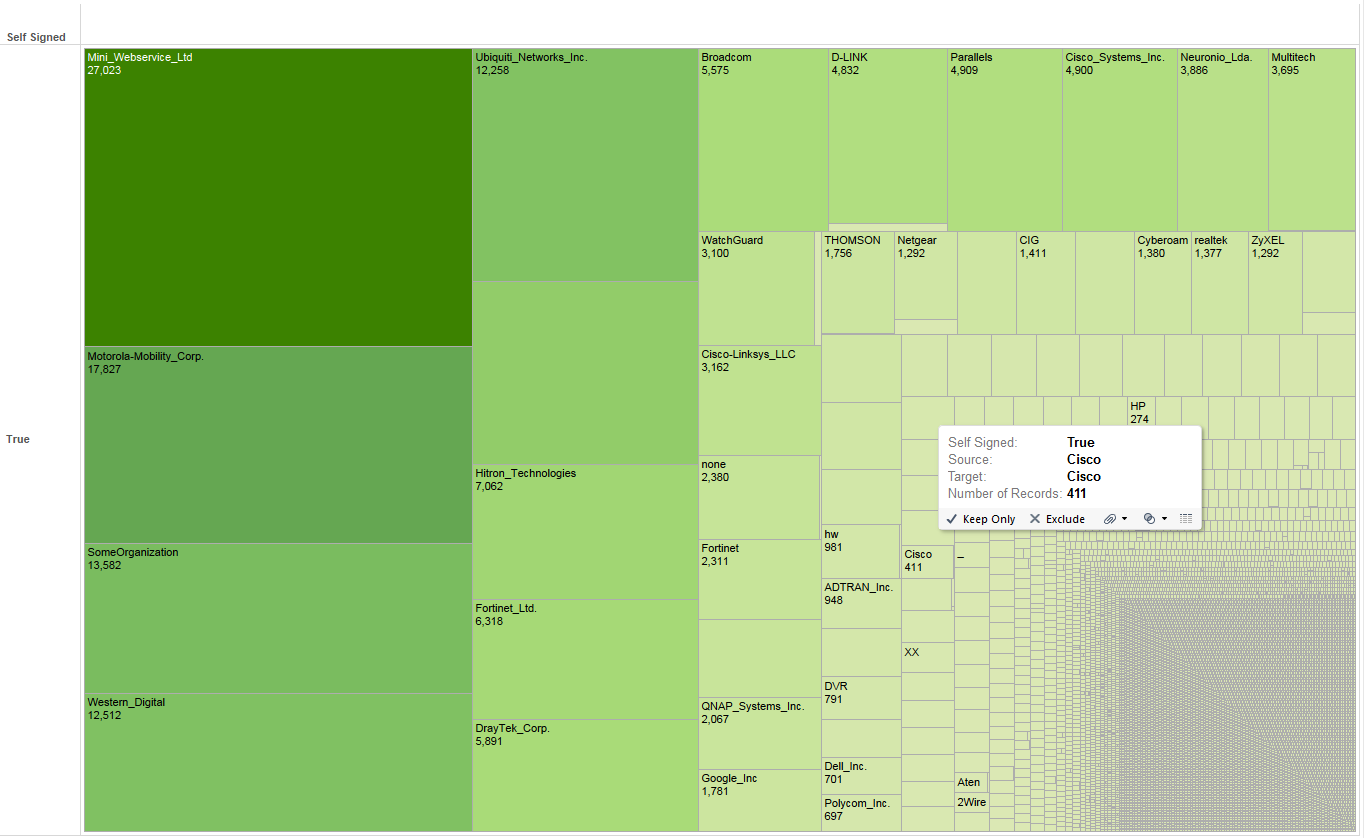
\includegraphics[scale=0.20]{./images/SelfSigned.png}
        \end{center}
\end{frame}

\begin{frame}[t,fragile]{Dyre malware and SSL fingerprint}
        \begin{itemize}
                \item Dyre malware contains a list of static IP addresses to reach as C\&C. What kind of C\&C?
        \end{itemize}
        \begin{lstlisting}[language=json,firstnumber=1]
{"5.44.15.70": ["C=US, ST=CA, L=San Jose, O=Ubiquiti Networks Inc., OU=Technical Support, CN=UBNT/emailAddress=support@ubnt.com"]}
{"93.184.71.88": ["C=US, ST=CA, L=San Jose, O=Ubiquiti Networks Inc., OU=Technical Support, CN=UBNT/emailAddress=support@ubnt.com"]}
        \end{lstlisting}
        \begin{itemize}
                \item The compromised Ubiquiti routers (with default password) were compromised to proxy SSL connections.
        \end{itemize}
\end{frame}

\lstdefinelanguage{brol}{
    basicstyle=\normalfont\ttfamily,
    numbers=left,
    numberstyle=\scriptsize,
    stepnumber=1,
    numbersep=8pt,
    showstringspaces=false,
    breaklines=true,
    frame=lines,
    basicstyle=\tiny,
    backgroundcolor=\color{background},
}

\begin{frame}[t,fragile]{How to find user of a specific software?}
     \begin{itemize}
             \item Who use MobileIron Mobile Device Management? More than 11000 certificates on a two-year period.
     \end{itemize}
      \begin{lstlisting}[language=brol]
c2ef4df6c7be287f78ae9178d65e8078f253cfb1,C=US, ST=California, L=Sunnyvale, O=MobileIron, OU=Support, CN=ActiveSyncProxyCA/emailAddress=support@mobileiron.com
5c10590f0e977c15805124ddc00f470383768b10,C=US, ST=California, L=Sunnyvale, O=MobileIron, OU=Support, CN=usslmmdmsecapp004.net.plm.eds.com/emailAddress=support@mobileiron.com
9ce9edf68ecbf59c746e0d3bbe6d98d72b65fed3,C=US, ST=California, L=Sunnyvale, O=MobileIron, OU=Support, CN=mbx-desat-otn.defdh.astrium.eads.net/emailAddress=support@mobileiron.com
b47ec8382624035448eebcf15a1cd402425ca661,C=US, ST=California, L=Sunnyvale, O=MobileIron, OU=Support, CN=ActiveSyncProxyCA/emailAddress=support@mobileiron.com
5190314e4590420e75a2e7b21c74b34255da0806,C=US, ST=California, L=Sunnyvale, O=MobileIron, OU=Support, CN=ats.patrizia.ag/emailAddress=support@mobileiron.com
      \end{lstlisting}
\end{frame}

\begin{frame}[t,fragile]{Detecting dynamic IP ranges?}
        \begin{itemize}
                \item SSL/TLS services are often running on dynamic IP ranges. Users use dynamic DNS. Dynamic ranges managed by ISP can be detected and associated users too.
        \end{itemize}
        \begin{lstlisting}[language=brol]
d53cc7380ed06c8b8ef0163952c9c534afad7ab8,CN=pino007.ath.cx
92bfef7362de7b381c723a2a352d54d82d49712a,CN=profinance.ath.cx
2cd0f2033c756222c976b631dba1a95a87aeadf9,CN=kschaub.ath.cx
c0de4fe83452046c0529b74f6081a39f82907746,CN=fferemote.ath.cx
b0d04a23ff6da2191d7b78f72352f1196802f61f,CN=hm01-server.Filmhotel.local, CN=localhost, CN=hm01-server, CN=companyweb, CN=filmhotel.ath.cx
a4b54adb780a5c9ea737399f9492f9f4dafc721d,CN=praxis-drciftci.ath.cx
77b89a57304256562ebfa42024fa9adeb304ad5a,CN=remote.mandk.ath.cx
        \end{lstlisting}
\end{frame}

\begin{frame}[t,fragile]{Popcorn time}
        \begin{lstlisting}[language=brol]
e4bd71c2e365b61b39d775ba43ef936a4fe9175c,C=Unknown, ST=Unknown, L=Unknown, O=Unknown, OU=Unknown, CN=*.*
1fc3a857a14ca15d3c37fdb2c8b7e0de01e4f0fd,C=IL, ST=Tel Aviv, O=Visonic Ltd., CN=*.*
397b25c864131bc78aff25622296171d60843318,C=IE, ST=Dublin, O=Fuck SSL Cartels, CN=*.nosmo.me/emailAddress=nosmo@nosmo.me
        \end{lstlisting}

\begin{itemize}
\item We can laugh at everything? Especially with this certificate proposed by 94.242.58.131
\end{itemize}
        \begin{lstlisting}[language=brol]
06892001be0854570546b1e609d33a5510290e3b,C=US, ST=California, L=Mountain View, O=GeoTrust Inc., OU=GeoTrust Global CA, CN=*.*

Issuer: C=US, ST=California, L=Mountain View, O=GeoTrust Inc., OU=GeoTrust Global CA, CN=*.*
Validity
      Not Before: May 19 09:54:04 2015 GMT
      Not After : May 16 09:54:04 2025 GMT
Subject: C=US, ST=California, L=Mountain View, O=GeoTrust Inc., OU=GeoTrust Global CA, CN=*.*

        \end{lstlisting}

\end{frame}


\begin{frame}[t, fragile]{Conclusion}
        \begin{itemize}
                \item Passive SSL helped us to get in contact with owners of vulnerable or abused systems.
                \item Passive SSL is an ongoing project and you can request access if do incident handling or security research\footnote{\url{https://www.circl.lu/services/passive-ssl/}}.
                \item Weird occurences in dataset lead to additional insights.
                \item Analysing the same dataset with different eyes improved analysis.
                \item Comparing different datasets can be independant verification of facts or proportion.
                \item Information visualisation can be used as a navigation strategy before deep diving.
        \end{itemize}
\end{frame}

\begin{frame}[t, fragile]{Q\&A}
        \begin{itemize}
                \item @blackswanburst - eireann.leverett@cantab.net
                \item @adulau - alexandre.dulaunoy@circl.lu
        \end{itemize}

\end{frame}

